\section{Introduction / Einführung}
Beispiele f\"ur Zitate: 	\cite{Schneier2004,Anderson2008,Eckert2007,Howard1998,Jaquith2007,Schneier2003}

\subsection{Szenario}
A concrete, but simple example from the \emph{financial services domain} is a generic trading process, e.g., in investment banking, where market data such as interest rates and ratings are retrieved from external agencies for deal pricing calculations (cf.~Figure~\ref{fig:screenshot}). Just by monitoring the message exchange between the bank and the agencies, an attacker can gain information about the amount of requests for the internal deal calculations, when the bank works on its deals, and so on. 

If more complex service compositions can be observed, e.g., if successful deals are processed by transaction services, attackers can also infer information about transactions closed successfully in general -- among which are also successfully closed deals. This is easily available, but very sensitive information that is not protected by the currently used Web service security technology. However, standard anonymity mechanisms are available for communication systems which could be used until dedicated solutions are available, i.e., taking into account the high Quality of Service (QoS) requirements of Web service communication. 

A concrete, but simple example from the financial services domain is a generic trading process, e.g., in investment banking, where market data such as interest rates and ratings are retrieved from external agencies for deal pricing calculations (cf.~Figure~\ref{fig:screenshot}). Just by monitoring the message exchange between the bank and the agencies, an attacker can gain information about the amount of requests for the internal deal calculations, when the bank works on its deals, and so on. If more complex service compositions can be observed, e.g., if successful deals are processed by transaction services, attackers can also infer information about transactions closed successfully in general -- among which are also successfully closed deals. This is easily available, but very sensitive information that is not protected by the currently used Web service security technology. However, standard anonymity mechanisms are available for communication systems which could be used until dedicated solutions are available, i.e., taking into account the high Quality of Service (QoS) requirements of Web service communication. 

\begin{figure}[tb]
	\centering
	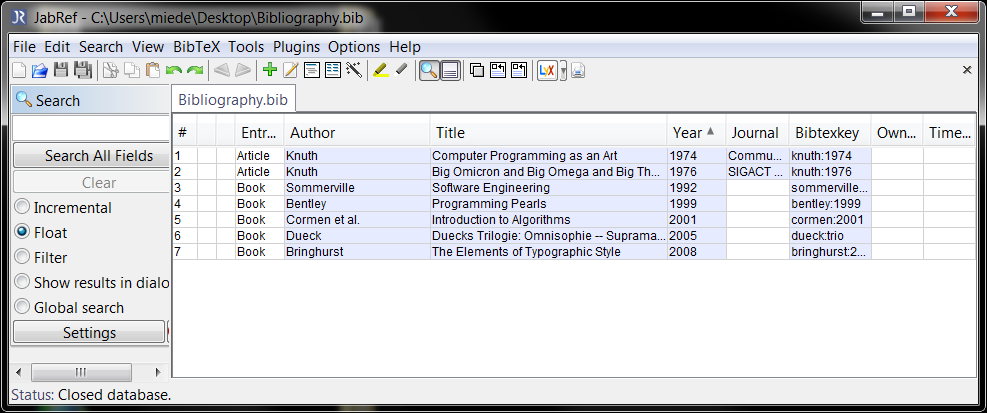
\includegraphics[width=\columnwidth]{gfx/jabref} %.5\textwidth
	\caption{Screenshots should be in PNG format, general photos in JPG, and diagrams etc. as PDF (vector).}\label{fig:screenshot}
\end{figure}


In total, we choose eleven different Web services from distinct and globally distributed providers as shown in Table~\ref{tab:wsdistr}. 
\begin{table}[tb]
	\centering
	\caption{Global distribution of Web service providers used for the experiments.}\label{tab:wsdistr}
	\begin{tabular}{ll}\toprule
		\emph{Country} & \emph{Web service provider} \\ \midrule
		USA & \texttt{www.webservicex.com} \\
		USA & \texttt{ws.cdyne.com} \\
		USA & \texttt{www.kbb.com} \\
		Australia & \texttt{national.atdw.com.au} \\
		Great Britain & \texttt{dw.sheetmusicdirect.com} \\
		The Netherlands & \texttt{artselect.artikelbeheer.nl} \\
		Canada & \texttt{netpub.cstudies.ubc.ca} \\ \midrule
		Russia & \texttt{www.cbr.ru} \\ 
		China & \texttt{www.sircweb.cn} \\
		Brazil & \texttt{ws.cronostelemetria.com.br} \\
		Germany & \texttt{mathertel.de} \\ \bottomrule
	\end{tabular}
\end{table}

Just by monitoring the message exchange between the bank and the agencies, an attacker can gain information about the amount of requests for the internal deal calculations, when the bank works on its deals, and so on. If more complex service compositions can be observed, e.g., if successful deals are processed by transaction services, attackers can also infer information about transactions closed successfully in general -- among which are also successfully closed deals.  


\begin{figure*}[t]
	\centering
	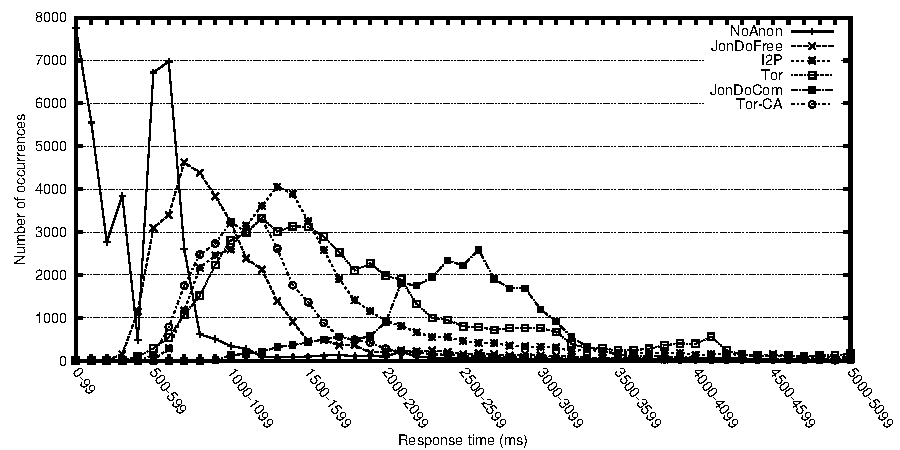
\includegraphics[width=\textwidth]{gfx/histo_allcurves} %.5\textwidth
	\caption{Overall number of measured response times per anonymity system.}\label{fig:histoall}
\end{figure*}


\section{Related Work / Stand der Technik}
A concrete, but simple example from the financial services domain is a generic trading process, e.g., in investment banking, where market data such as interest rates and ratings are retrieved from external agencies for deal pricing calculations (cf.~Figure~\ref{fig:screenshot}). Just by monitoring the message exchange between the bank and the agencies, an attacker can gain information about the amount of requests for the internal deal calculations, when the bank works on its deals, and so on. If more complex service compositions can be observed, e.g., if successful deals are processed by transaction services, attackers can also infer information about transactions closed successfully in general -- among which are also successfully closed deals. This is easily available, but very sensitive information that is not protected by the currently used Web service security technology. However, standard anonymity mechanisms are available for communication systems which could be used until dedicated solutions are available, i.e., taking into account the high Quality of Service (QoS) requirements of Web service communication. 


\section{\dots}
A concrete, but simple example from the financial services domain is a generic trading process, e.g., in investment banking, where market data such as interest rates and ratings are retrieved from external agencies for deal pricing calculations (cf.~Figure~\ref{fig:screenshot}). 


\section{Summary and Outlook / Zusammenfassung und Ausblick}
A concrete, but simple example from the financial services domain is a generic trading process, e.g., in investment banking, where market data such as interest rates and ratings are retrieved from external agencies for deal pricing calculations (cf.~Figure~\ref{fig:screenshot}). Just by monitoring the message exchange between the bank and the agencies, an attacker can gain information about the amount of requests for the internal deal calculations, when the bank works on its deals, and so on. If more complex service compositions can be observed, e.g., if successful deals are processed by transaction services, attackers can also infer information about transactions closed successfully in general -- among which are also successfully closed deals. This is easily available, but very sensitive information that is not protected by the currently used Web service security technology. However, standard anonymity mechanisms are available for communication systems which could be used until dedicated solutions are available, i.e., taking into account the high Quality of Service (QoS) requirements of Web service communication. 

